\documentclass[fleqn,12pt]{wlscirep}

\newcommand{\todo}[1]{\textcolor{gray}{#1}}
\newcommand{\fixme}[1]{\textcolor{red}{#1}}
\newcommand\note[1]{\mbox{}\marginpar{\footnotesize\raggedright\hspace{0pt}\color{blue}\emph{#1}}}
\usepackage{gensymb}
\usepackage{lineno}
\linenumbers
\usepackage{graphicx}
\graphicspath{ {images/} }


\usepackage{hyperref}
\hypersetup{
     colorlinks   = true,
     citecolor    = black,
     linkcolor = black,
     urlcolor     = black
}

\usepackage{parskip}
\setlength{\parskip}{6pt}
\setlength{\parindent}{0pt}
\renewcommand{\baselinestretch}{1.1} 

\usepackage[font={small, singlespacing}]{caption}

\usepackage{wrapfig}

\title{Diffusion-driven enhancement of the antibiotic resistance selection window}

\author[1,*]{Ayari Fuentes-Hern\'andez}
\author[1,$\dag$]{Anastasia Hern\'andez-Koutoucheva}
\author[1,$\dag$]{Al\'an F. Mu\~noz}
\author[1,$\dag$]{Ra\'ul Dom\'inguez Palestino}
\author[1]{Rafael Pe\~na-Miller}
\affil[1]{  \, Laboratorio de Biolog\'ia Sint\'etica y de Sistemas, Centro de Ciencias Gen\'omicas, Universidad Nacional Aut\'onoma de M\'exico, 62210, Cuernavaca, M\'exico}
\affil[*]{Corresponding author: ayarifh@ccg.unam.mx}
\affil[$\dag$]{These authors contributed equally to this work}

\keywords{antibiotic resistance, spatial structure, mathematical modelling, 3D printing}

\begin{abstract}
The current crisis of antimicrobial resistance in clinically-relevant pathogens has highlighted our limited understanding of the ecological and evolutionary forces that drive drug resistance adaptation. For instance, although  human tissues are highly heterogeneous, most of our mechanistic understanding about antibiotic resistance evolution is based on constant and well-mixed environmental conditions.
A consequence of considering spatial heterogeneity is that, even if antibiotics are prescribed at high dosages, the penetration of drug molecules through tissues inevitably produces antibiotic gradients, exposing bacterial populations to a range of selective pressures and generating a dynamic fitness landscape that changes in space and time.   
In this paper, we will use a combination of mathematical modelling and computer simulations to study the population dynamics of susceptible and resistant strains competing for resources in a network of micro-environments with varying degrees of connectivity. Our main result is that highly-connected environments increases diffusion of drug molecules, enabling resistant phenotypes to colonize a larger number of spatial locations. We validated this theoretical result by culturing fluorescently-labelled {\em Escherichia coli} in 3D-printed devices that allow us to control the rate of diffusion of antibiotics between neighbouring compartments and quantify the spatio-temporal distribution of resistant and susceptible bacterial cells.  \vspace{-20pt}
\end{abstract}
\begin{document}

\flushbottom
\maketitle
\vspace{-10pt}
\thispagestyle{empty}

%%%%%%%%%%%%%%%%%%%%%%%%%%%%%%%%%%%%%%%%%%%
\section*{Introduction}

The introduction of antimicrobial substances as therapeutic agents has had a dramatic effect in decreasing mortality and morbidity associated with infectious diseases. However, the indiscriminate use of these substances, in conjunction with the accelerated rate of adaptation exhibited by pathogenic bacteria, has dramatically reduced the efficacy of antimicrobial therapies and presents us with the possibility of a health-care crisis of catastrophic dimensions \cite{WHO2014}. In this context, it is necessary to invest in the discovery of new drugs\cite{AMR2015} and to reduce the use of antimicrobial substances, both in the clinic\cite{Lee2013} and elsewhere\cite{Meek2015}, but also to increase our understanding about the complex interaction between antibiotics, bacteria and hosts.

Of course, the ultimate goal of antimicrobial therapy is to drive a pathogenic population to extinction, so antibiotics must be prescribed at concentrations high enough for bacterial cells to die. Even if complete clearance of pathogens cannot be achieved, conventional wisdom states that high drug dosages suppress growth of the bacterial population and adjuvate the immune system to control the infection. Another benefit of maximizing the inhibitory effect of antibiotics, is that, in principle, the mutational supply is reduced and therefore the probability that an individual in the population acquires an antibiotic-resistance mutation is lower\cite{Stratton2003} (although studies have shown that mutation rates can be density-dependant \cite{Richards2017} and increased in the presence of antimicrobial substances\cite{Galhardo2007}).

But aggressive antibiotic protocols can accelerate the rate of adaptation, for instance by suppressing susceptible competitors and releasing resources that promote growth of the resistant subpopulation\cite{PenaMiller2013}. Motivated by the evident failure of the current `{\em hit early, hit hard}' prescription strategy\cite{Read2011}, a series of theoretical and experimental studies have argued that antimicrobial therapies should consider resistance management instead of focusing exclusively in pathogenic clearance, for example by using shorter \cite{Geli2012} and less aggressive \cite{Kouyos2014} treatments, multidrug combination therapies\cite{Hegreness2008,Baym2016}, sequential treatments \cite{Kim2014,Imamovic2013,FuentesHernandez2015} and increasing drug appropriateness with better point-of-care diagnostic tests \cite{Beardmore2017,McAdams2018}.

Another problem associated with the use of high doses of antibiotics is that, even if a lethal drug concentration is administered, a heterogeneous spatial structure will produce an antibiotic gradient and thus expose the pathogenic bacteria to a range of selective pressures in favour of resistance.
Indeed, it is well known that the therapeutic use of antibiotics sees {\em in vivo} drug concentrations sweep from high-concentrations downwards during treatment (with a considerable time spent at low drug concentrations\cite{PKPD}, producing low-dose sanctuaries that have been observed in bacterial \cite{Deresinski2009} and viral infections \cite{Solas2003}, promoting the evolution of antibiotic resistance\cite{Moreno2015}. For this reason, previous studies have focused on evaluating the effect of sub-lethal doses in the evolution of drug resistance \cite{Nosanchuk2014} and in modulating virulence factors \cite{Arnoldini2014}, showing that selection for resistance can occur at very low antibiotic doses  \cite{Gullberg2011,Andersson2014} and that antibiotic gradients can accelerate the rate of drug-resistance adaptation \cite{Hermsen2012,Greulich2012,Zhang2011}. Similarly, convection \cite{Gralka2017} and cell migration \cite{Baym2016} can lead to increases in drug resistance through sequential adaptive steps in space and time. 

As the ecological and evolutionary dynamics of a microbial community depend on the genotypic and functional complexity of the population and their interaction with the environment\cite{Tecon2019}, then the chemical composition of the media is a key driver of microbial ecological and evolutionary dynamics. Crucially, this is modified by the physical properties of the environment, for instance its temperature\cite{Tenaillon2012} and humidity\cite{Zoz2016}, but also by  structural properties like geometry\cite{Lowery2018} and porosity\cite{Or2007}.  In this paper, we will argue that the connectivity between different spatial locations is directly responsible for the distribution of antibiotics in the environment, thus producing a range of selective pressures in favour of resistance.

In short, we will use a population dynamics model to argue that selection for resistance is correlated with the degree of connectivity of the environment, both in a linear array of connected micro-environments and also in networks with different topological properties. This prediction will be validated empirically using an experimental model system based on spatially-explicit culture devices built using computer aided design software and 3D printing technology. These devices allow us to control the rate of diffusion of drug molecules between neighbouring micro-environments, while quantifying spatio-temporal changes in the relative frequency of fluorescently-tagged resistant and susceptible {\em Escherichia coli} strains.

%%%%%%%%%%%%%%%%%%%%%%%%%%%%%%%%%%%%%%%%%%%
\section*{Results}

\subsection*{Competitive fitness in a range of drug concentrations}

In this paper we will use two strains of \textit{E. coli} MC4100\cite{Chait2007,Chait2010}: \textsc{Wcl}, a strain carrying $Km^R$, a gene that provides resistance to the aminoglicocide antibiotic Kanamycin, and \textsc{Gby}, a susceptible strain that lacks $Km^R$. All experiments were conducted using M9 minimal media supplemented with 0.4\% of glucose and 0.2\%  of casaminoacids. 
Furthermore, each bacterial strain is tagged with a different fluorescent marker under a chromosomal constitutive promoter (\textsc{Wcl} with CFP and \textsc{Gby} with YFP), allowing us to use a fluorescent spectrophotometer to quantify the intensities of both fluorescent channels and use this information to estimate the relative abundances of each strain in a mixed population.

Our main objective is to identify the range of drug concentrations where antibiotic resistance is positively selected for. To achieve this goal, we first need to evaluate the fitness advantage associated with carrying a drug-resistant gene, a property that can be estimated using a pair-wise competition experiment that directly compares the fitness of the drug-resistant genotype with respect to the susceptible strain. This can be achieved using a standard protocol in experimental microbiology that consists on growing both strains in controlled environmental conditions for $T$ units of time (usually 24 hours), and then estimating the relative abundances of each bacterial subpopulation using a fluorescent spectrophotometer, a flow cytometer or replica plating with selective media. From the relative frequency of each strain at the end of the experiment we can then define the following {\em relative fitness} coefficient:
\begin{equation}
\phi_r := \phi_r(A)= \frac{\ln(B_s(T)/B_s(0))}{\ln(B_r(T)/B_r(0))},\label{eq:phi}
\end{equation}\vspace{-0pt}
where $B_r(t)$ and $B_s(t)$ denote the densities of resistant and susceptible strains, respectively, and $A$ the environmental concentration of the antimicrobial substance (in our case, Kanamycin).  For the purpose of this paper, we will consider that $B_r(0)=B_s(0)$, an assumption that allows us to estimate $\phi_r(A)$ based only in observations about the state of the system at the end of the experiment. 

Figure 1B shows the optical densities of both bacterial strains after 24 hours of growing in rich media (LB) in the absence of antibiotics, both in co-culture and in isolation.  Note that growth of the resistant mono-culture (cyan bar) is lower than that of the susceptible bacteria (yellow), implying that Kanamycin resistance is associated with a fitness burden in drug-free environments\cite{Melnyk2015}. 
As a result, the susceptible strain has a higher competitive fitness than the resistant sub-population at low antibiotic concentrations, a feature represented by the inequality $\phi_r<1$.



In contrast, if the concentration of antibiotic is high, then the advantage of carrying a resistance mutation outweighs its fitness burden and therefore $\phi_r(A)$ is a monotonously increasing function of antibiotic dose (see Figure 1A).  If we denote with $A_{MSC}$ the antibiotic concentration such that $\phi_r(A) > 1$ for all $A > A_{MSC}$, then we can identify the range of drug concentrations whereby resistance is positively selected for. This critical concentration is referred to in the literature as the {\em Minimal Selection Concentration}\cite{Gullberg2011} (MSC).

%%%%%%%%

\clearpage
%%%%%%%%
%%Figure 1 

\begin{wrapfigure}{r}{0.5\textwidth}\centering
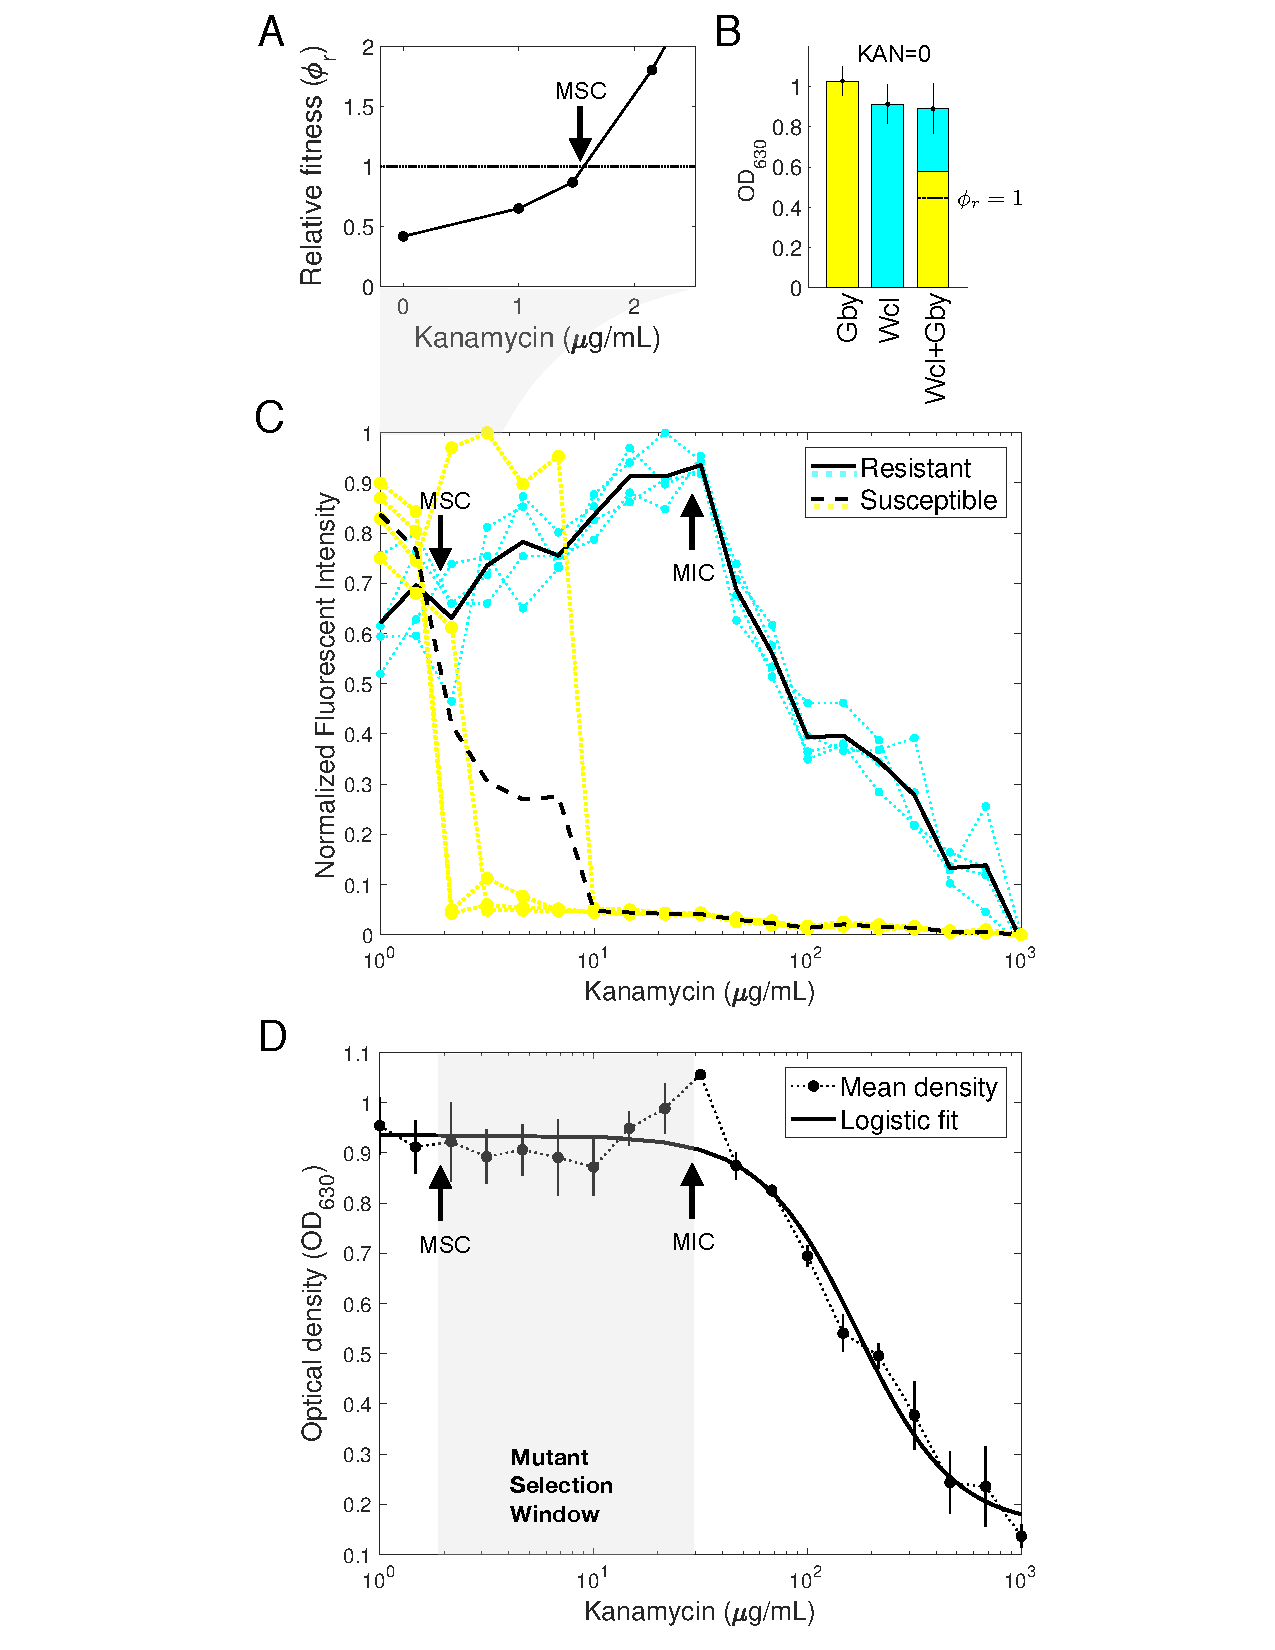
\includegraphics[width=0.9\linewidth]{figures/Figure1.pdf}
\caption{\footnotesize Effect of antibiotic concentration in a competition experiment between resistant (\textsc{Wcl}, CFP) and susceptible (\textsc{Gby}, YFP) strains. A) Relative fitness as a function of Kanamycin concentration, in co-culture. B) Optical density of each strain, on isolation and co-culture. Growth of the susceptible strain is larger compared to the resistant subpopulation. C) Normalized fluorescent intensity measured under a range of drug concentrations.  D) Mean optical density of the co-culture obtained in a dose-response experiment where the total bacterial density decreases as the concentration of antibiotics increases (C). Concurrently, the fraction of the population that is drug-resistant becomes larger (D). }
\label{fig:figure1}
\end{wrapfigure}


In order to study how the local strength of selection for resistance changes in an antibiotic gradient, we use a dose-response experiment that consists on growing cells under increasing drug concentrations and measuring bacterial densities or maximal growth rates in a fixed time interval. This assay is routinely used in medical microbiology to estimate drug concentrations that completely inhibit growth of a specific clinical isolate and, for this reason, dose-response experiments are usually performed with mono-cultures. In our experiments, we inoculate the dose-response experiment with both strains, with the aim of computing $\phi_r(A_i)$ for a range of drug concentrations $A_1 < A_2 < \dots < A_i < \dots < A_n$.


Another critical antibiotic concentration is known as the {\em Minimum Inhibitory Concentration} (MIC), defined as the drug concentration such that bacterial growth is completely suppressed. In general, the shape of dose-response curves can be approximated with a logistic equation. Indeed, Figure 1D shows that total bacterial density remains constant at sub-MIC concentrations, but relative abundances of each subpopulation change as a function of dose, with $B_r$ increasing in frequency as the concentration of drug increases.  The region in drug-space where bacterial growth is still observed ({\em i.e.} $\frac{d }{dt}B_r>0$) and drug resistance is under positive selection ({\em i.e.} $\phi_r(A)>1$), is known as the {\em Mutant Selection Window} (MSW) \cite{Drlica2007}. 

An interesting observation obtained by comparing Figures 1C and 1D, is that the MIC of the co-culture corresponds to the MIC of the resistant subpopulation, while the susceptible strain has, by definition, a lower MIC.  Interestingly, in our experiments, bacterial density seems to be maximized at intermediate drug concentrations, a feature that has been reported previously\cite{Eagle1948} and can have many causes, including $B_r$ growing without competition at intermediate drug concentrations \cite{PenaMiller2014}. Indeed, Figure 1C and 1D show that there is a range of concentrations where $B_s$ has already gone extinct, but the concentration is not high enough to suppress growth of the resistant subpopulation.  Note that, in clinical settings, this is the region of drug-space that we would like to avoid in order to promote the evolution of drug resistance.

%%%%%%%%%%%%

\subsection*{Modeling drug-resistance population dynamics}

Previous studies have used a {\em top-down} approach and postulated pharmacodynamic models derived from fitting dose-response curves with Hill functions\cite{Engelstadter2014,Regoes2004}.  Instead, here we will use a {\em bottom-up} approach that explicitly considers the concentrations of limiting resource and antibiotics present in the environment, with the aim of evaluating the population dynamics between susceptible and resistant bacterial types that emerges in response to different environmental conditions. In the following section we will discuss how to include the spatial component into the model, but first let us assume that the environment is well-mixed and, therefore,  the interaction between bacterial cells and abiotic molecules follows a mass action kinetics so we can model temporal changes in bacterial abundances using a system of ordinary differential equations.

Although clearly a possibility, for the purpose of this paper we will not consider that susceptible cells can acquire drug resistance through stochastic mutations or horizontal gene transfer.  The reason for this assumption is that we are mainly interested in studying the ecological dynamics of the system after a resistant mutant appears in the population. Therefore, both in our numerical simulations and in the experiments discussed later in this paper, we will consider that both strains are {\em a priori} present in the system the moment the antibiotic is deployed and quantify the strength of selection for resistance, $\phi_r(A)$), in response to a range of antibiotic concentrations.  

First, let us represent the concentration of a limiting resource present in the environment with the variable $R(t)$. Then uptake of resources into each cell can be modeled with a non-linear saturating resource uptake function that depends on $R(t)$:
\begin{equation}
 U_*(R(t))= \frac{\mu^*_{max}R(t)}{K_m^*+R(t)},
\end{equation}
where $\mu^*_{\max}$ and $K_m^*$ denote the maximum uptake rate and the half-saturation constants, respectively, of bacterial type $B_*$.

Now let us suppose that, at time $t$, the environment contains an antibiotic at a concentration that we will denote $A(t)$. In particular, we will consider an antibiotic with a bacteriostatic mode of action, namely that it inhibits bacterial growth by interfering with protein translation, DNA replication, or other aspects of bacterial cellular metabolism. As mentioned before, in the experiments presented in this paper we are using Kanamycin, an aminoglycocide that binds to the 30S subunit of the ribosome, thereby suppressing bacterial protein synthesis and inhibiting growth.  Therefore, we will model growth inhibition with a monotonously decreasing function, such that $\gamma(A(t)) \geq 0$ for all $A$, and with $\gamma(0)=1$ in the absence of antibiotic, for instance,
\[
\gamma(A)=1-\frac{k_1 A}{1+k_2 A},
\]
where parameters $k_1$ represent the cell's affinity for the antibiotic and $k_2$ the maximal growth inhibition by the bacteriostatic drug\cite{PenaMiller2011}. Also, we will consider that $\alpha_s$ and $\alpha_r$ are parameters that represent the inactivation of drug molecules for each bacterial strain as a result of their binding with the cellular targets.

Then bacterial growth rate of bacterial type $B_*$ can be modeled as the resource uptake function multiplied by the inhibition coefficient, $G_*(R,A) =\rho_* \cdot \gamma_*(A) \cdot U_*(R)$, where $\rho_*$ denotes a resource conversion coefficient that represents the efficiency of each subpopulation in converting resource molecules into biomass.

So, if $x(t)=(R(t),A(t),B_s(t),B_r(t))$ represents the state of the system, the system of equations that describe its temporal dynamics can be written as:
\begin{subequations}
\begin{align}
 \frac{dR}{dt}=&-U_s(R)B_s-U_r(R)B_r \label{odes1} \\
 \frac{dA}{dt}=& - A(\alpha_s B_s   + \alpha_r B_r) \label{odes2}\\
 \frac{dB_s}{dt}=&  G_s(R,A)  B_s \label{odes3}\\
 \frac{dB_r}{dt}=&  G_r(R,A)  B_r \label{odes4}
\end{align}
\label{eq:ode}
\end{subequations}
with initial conditions $x(0)=(R^0, A^0, B_{s}^0, B_{r}^0)$. 

Figure \ref{fig:figure2} shows numerical simulations of this model with different initial drug concentrations and parameter values described in Table 1 (solved using standard ODE solvers in Matlab). Note how at low antibiotic concentrations, $B_s$ has a higher growth rate than $B_r$ and therefore the yellow area is larger than the blue area. As the concentration of antibiotic increases, so does the competitive fitness of the resistant strain until eventually the susceptible strain is no longer able to grow and the population is entirely composed of resistant cells (blue area). At very high drug concentrations, neither of the strains can grow and the bacterial population is completely suppressed.

%%%%%%%%
%%Figure 2
\begin{figure}[ht!]
\centering
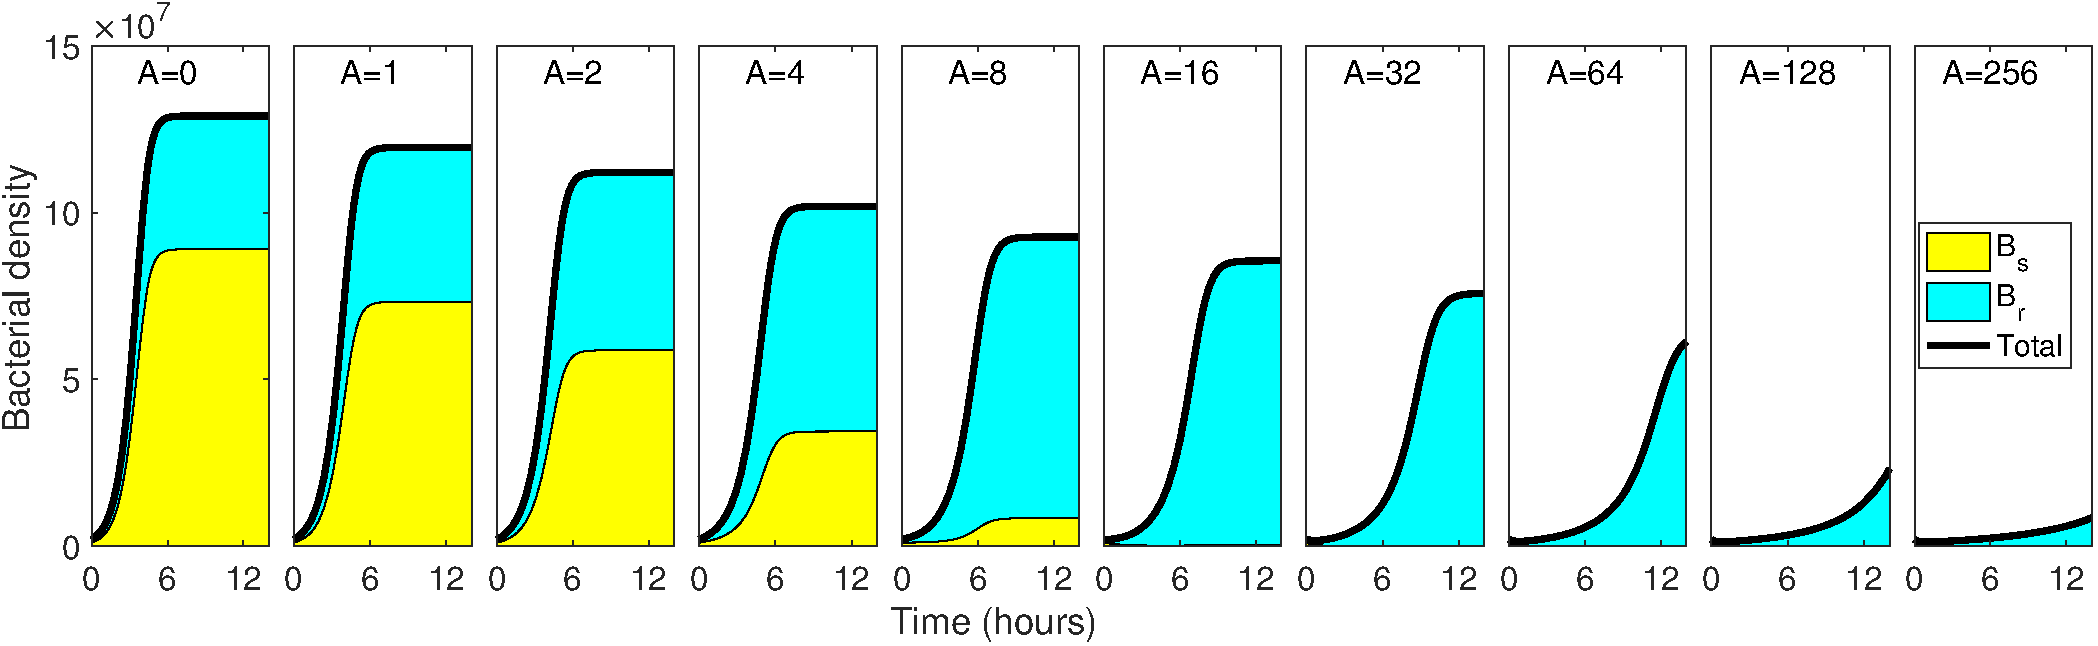
\includegraphics[width=1\linewidth]{figures/Figure2.pdf}
\caption{\footnotesize Numerical simulations of equations \ref{eq:ode}a-d with parameters described in Table 1. Each box shows a plot of bacterial density as a function of time (black line), with the density of resistant and susceptible sub-populations represented as stacked areas ($B_r$ in blue and $B_s$ in yellow). The environmental concentration of antibiotic doubles from left to right. We notice that, as expected, total bacterial density decreases as the concentration of antibiotic is incremented, but the frequency of resistance in the population is positively correlated with antibiotic dose.}
\label{fig:figure2}
\end{figure}
%%%%%%%%


%%%%%%%%%%%%
\subsection*{Modelling diffusion of antibiotics in connected micro-environments}

The model presented in the previous section assumes a uniform distribution of cells and abiotic molecules in the environment. This is, of course, a simplification, as natural environments like the human body are not homogeneous, but instead can be approximated with a series of discretely-distributed compartments\cite{Kepler1998}. 

It is known that  complex population dynamics can emerge from the mosaic of selective pressures imposed by a spatially structured environment, with separate locations selecting for specific gene variants \cite{Baquero1997}. Previous studies have also shown that drugs have characteristic penetration profiles through the tissue, thus creating antibiotic gradients and exposing bacterial populations to a range of antibiotic concentrations\cite{Moreno2015} and, as a result, producing dynamic drug resistance fitness landscapes \cite{Mira2015,Engelstadter2014}.

For the purpose of this paper we will consider that the environment consists of a network of connected micro-environments, each occupied by a polimicrobial community composed of susceptible and resistant strains. We will consider that abiotic substances (e.g. antibiotics and glucose) can diffuse between adjacent micro-environments, but with limited movement of cells between neighbouring colonies.  This is a strong assumption, but one that will allow us to argue that, even without considering cell migration, selection for resistance is enhanced in environments with a high degree of connectivity.

So, let us define $E$ as the spatial location where a group of cells interact with the extracellular environment. We will refer to this quasi-homogeneous region as a micro-environment or a compartment.  
Then we can model the population dynamics that occurs in each compartment using Equations (\ref{odes1}-\ref{odes4}), but with drug molecules diffusing between adjacent micro-environments.  
Therefore if $\delta_A$ represents the antibiotic diffusion rate and $\sigma_{i,j}$ the degree of connectivity between compartments $E^i$ and $E^j$, then the concentration of antibiotic in $E^i$ can be denoted by $A^i$ and modeled by the following differential equation:
\begin{equation}
\frac{dA^i}{dt}= - A^i(\alpha_s G_s(R^i) + \alpha_r G_r(R^i)) + \sum_{n=1}^N \sigma_{i,n} (A^n-A^i)\delta_A,  \label{eq:odeA}
\end{equation}
where $N$ represents the total number of micro-environments in the system ($\sigma_{i,j}=0$ when $E^i$ and $E^j$ are not connected). Similarly, we will also consider that resources can diffuse between micro-environments at a rate $\delta_R$. Therefore the differential equation that describes the rate of change of resource concentration in $E^i$ is
\begin{equation}
\frac{dR^i}{dt}= -U_s(R^i)B_s^i-U_r(R^i)B_r^i   + \sum_{n=1}^N \sigma_{i,n} (R^n-R^i)\delta_R.\label{eq:odeR}
\end{equation}

We would expect that, if a lethal concentration of antibiotic is deployed in a node of the network, the antibiotic concentration in a different location (and thus the strength of selection if favour of the resistant subpopulation in that micro-environment), will depend on the drug concentration used, but also on the distance to the antibiotic source.  

%%%%%%%%%%%%%%%%%%%%%%%%%%%%%%%%%%%%%%%%%%%

\subsection*{Dynamics of drug resistance in antibiotic gradients}

In order to evaluate how the degree of connectivity of the network correlates with the overall strength of selection for resistance, first we will consider that the environment is composed of a linear array of connected micro-environments. We will then solve numerically Equation \ref{eq:ode}a-d to evaluate the population dynamics that emerges in each micro-environment in response to an antibiotic gradient.  For simplicity, we will consider that all consecutive micro-environments are at the same distance of each other, that is $\sigma_{i,i+1} \equiv \sigma$. In contrast, $\sigma_{i,j} \equiv 0$ if compartments $E_i$ and $E_j$ are not consecutive.

As we are using a lethal antibiotic concentration, in the vicinity of the location where the drug was applied, bacterial growth was completely inhibited. In contrast, micro-environments far away from the drug source present very low antibiotic concentrations and thus susceptible bacteria grow until carrying capacity. These low-dose compartments are referred to in previous studies as drug sanctuaries \cite{Moreno2015}. At intermediate drug concentrations, however, the resistant subpopulation has a fitness advantage over the susceptible strain, $\phi_r>1$.

%%%%%%%%
%%Figure 3
\begin{figure}[ht!]
\centering
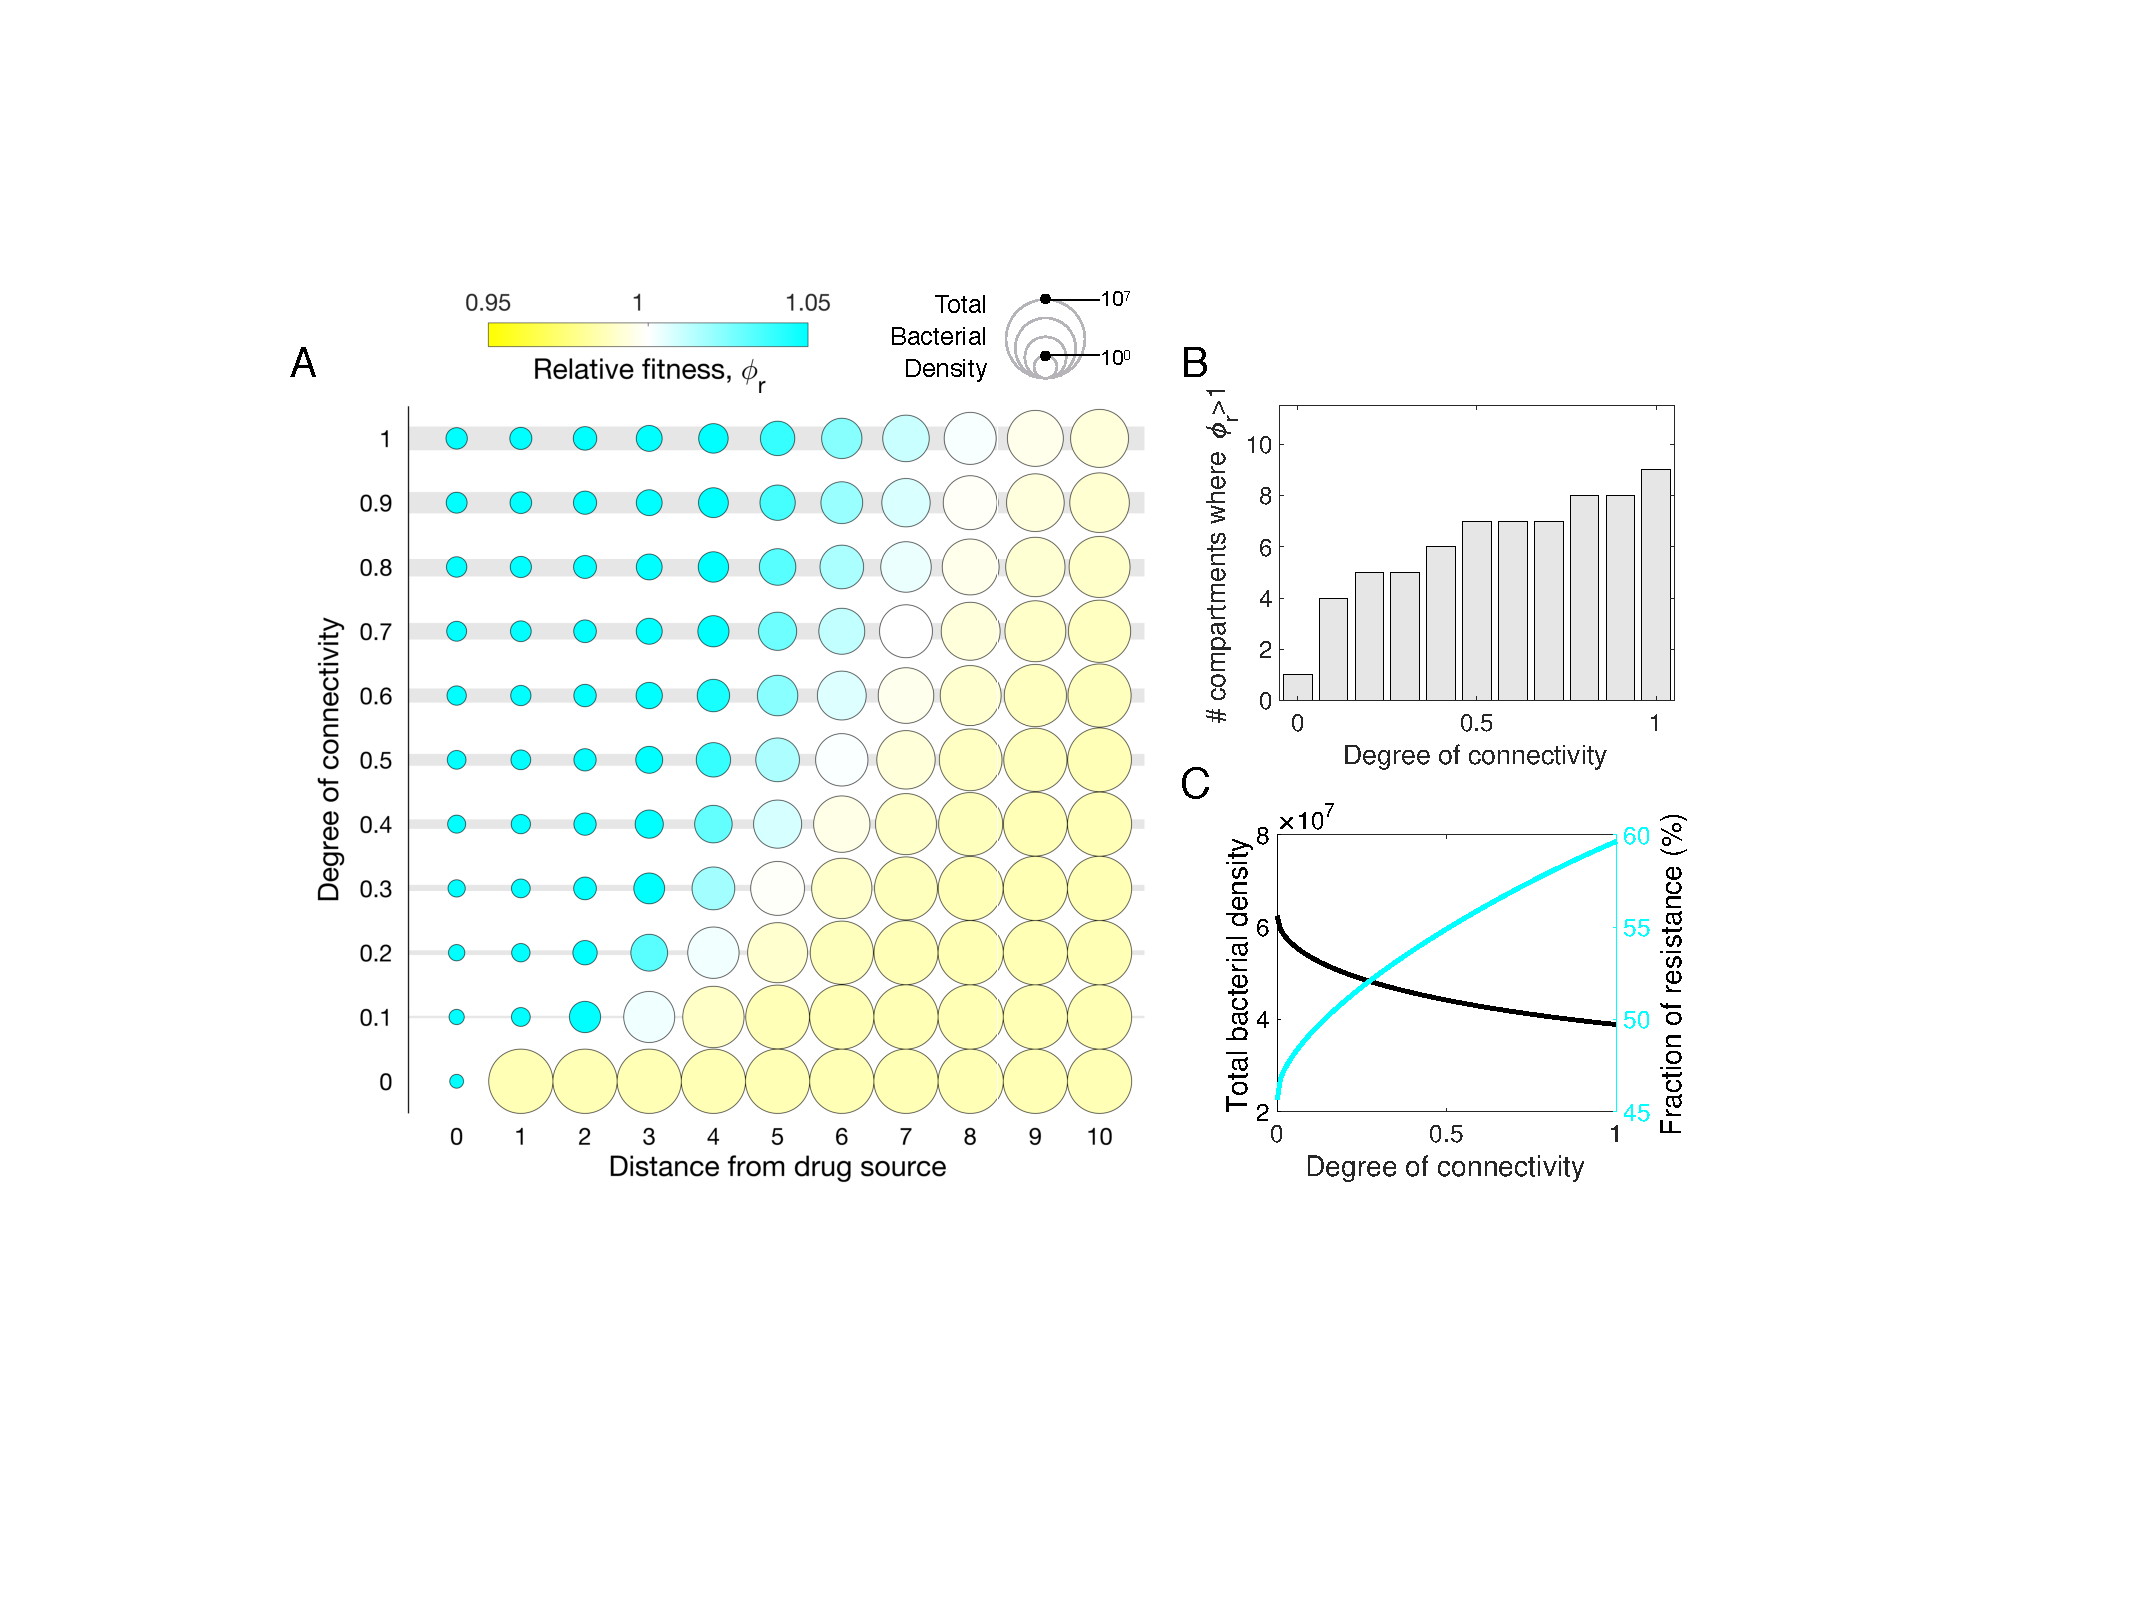
\includegraphics[width=1\linewidth]{figures/Figure3.pdf}
\caption{\footnotesize Numerical simulations of micro-environments with varying degrees of connectivity in a linear array.  A) Population dynamics of resistant and susceptible bacteria in different micro-environments. The diameter is proportional to the total bacterial density, while the relative fitness measured at the end of the experiment is color-coded (yellow represents that susceptible bacteria have a higher fitness and cyan that antibiotic resistance is positively selected for).  Each row corresponds to a different degree of connectivity (illustrated as a change on width), from no connection (bottom row) to a high-degree of connectivity (top row).  A lethal dose of antibiotics is deployed in the left-most column and hence, the horizontal axis represents the distance to the drug source. B) Proportion of micro-environments where the resistant bacteria have a higher fitness that the susceptible subpopulation (relative fitness >1). Note how, as the degree of connectivity increases, the number of compartments where resistant cells are selected for also increases. C) Total bacterial density as a function of connectivity degree. Although a monotonously decreasing function is observed (black line), the fraction of resistant cells in the population increases (cyan line). }
\label{fig:figure3}
\end{figure}
%%%%%%%%
\hspace{20pt}

Note that although the total concentration of antibiotic used is the same in all our numerical experiments, the number of micro-environments where $\phi_r>1$, that is the Mutant Selection Window, is higher in environments with high degree of connectivity. This is illustrated in Figure \ref{fig:figure3}A, where it shows that if we increase $\sigma$, the number of compartments where $\phi_r>1$ (blue circles) increases. Indeed, Figure \ref{fig:figure3}B shows that the number of micro-environments where the resistant strain outcompetes the susceptible subpopulation appears to be positively correlated with the degree of connectivity of the environment. 
Also, as a result of more antibiotic diffusing out of the source into the neighbouring compartments, the total bacterial density observed in all compartments decreases as we increase $\sigma$.  This in turn is correlated with an increase in the total frequency of resistance in the population, as illustrated in Figure \ref{fig:figure3}C.

%%%%%%%%%%%%

To investigate whether the enhanced diffusion of antibiotics produces increased selection for resistance, we will probe {\em in vitro} how antibiotic gradients modulate the fitness landscape of a population of resistant and susceptible bacteria. In particular, first we will consider a linear array of connected micro-environments with a lethal dose of antibiotic deployed in a single node. As expected, the antibiotic diffuses to the adjacent compartments, thus producing a drug gradient. Note that we can modify the gradient formed by increasing the connectivity between adjacent nodes.

It was recently shown that 3D printing can be performed in sterile conditions\cite{Neches2016}, so we designed a protocol that implements gradient devices printed in polylactic acid (PLA). In particular, we printed a linear array of micro-environments connected through channels that restrain movement of bacterial cells, but allow diffusion of antibiotic molecules between connected compartments (see Figure \ref{fig:figure4}A for an illustration of these devices). 
To characterize the gradient formed on these micro-environments, we printed a series of devices composed of wells connected through channels of different widths ($1$, $3$, and 5 mm) and filled each well with $200 \mu$L of soft M9 agar. We then applied a fluorescent dye to the first well and, using a fluorescence imaging system, estimated the concentration of dye in each compartment. As expected, antibiotic diffused out of the antibiotic source and a gradient was formed after 48 hours (illustrated in Figure \ref{fig:figure4}B).  

Once we established that the 3D-printed device can produce different gradients depending on the width of the channels, we then proceeded to produce an antibiotic gradient by filling the first well of each device with soft M9 agar and $50 \mu$g/ml of Kanamycin. We allowed the plate dry and then filled the rest of the wells with 200$\mu$L of soft M9 agar (without antibiotic) and placed the device at $4^{\circ}$C for 48 hrs for the drug gradient to form. 

The competition assay consisted in inoculating each well in the device with 10 $\mu$L of bacterial culture (on a mixture of 1:1 ratio of susceptible and resistant bacteria) and placing the device inside a petri dish, sealing it with parafilm and incubating it at $30^\circ$C for 24 hrs. As a control we also used a susceptible, non-fluorescent {\em E. coli} MG1655 strain.  In order to characterize and calibrate the profile of fluorescence generated by each genotype, we inoculated each strain in isolation and measured the fluorescence intensity observed using different optical configurations.  As expected, Figure \ref{fig:figure4}C shows that \textsc{Gby} can be detected using YFP filters and \textsc{Wcl} with CFP filters.  When cells are in co-culture, we detected fluorescence in both channels and use the maximum and minimum fluorescence observed by each strain grown in isolation to normalize the fluorescence of the mixed population (see Methods for experimental details).  We argue that the obtained relative fluorescence is a proxy for the relative abundances of each strain in the population.  

%%%%%%%%
%%Figure 4
\begin{figure}[ht!]
\centering
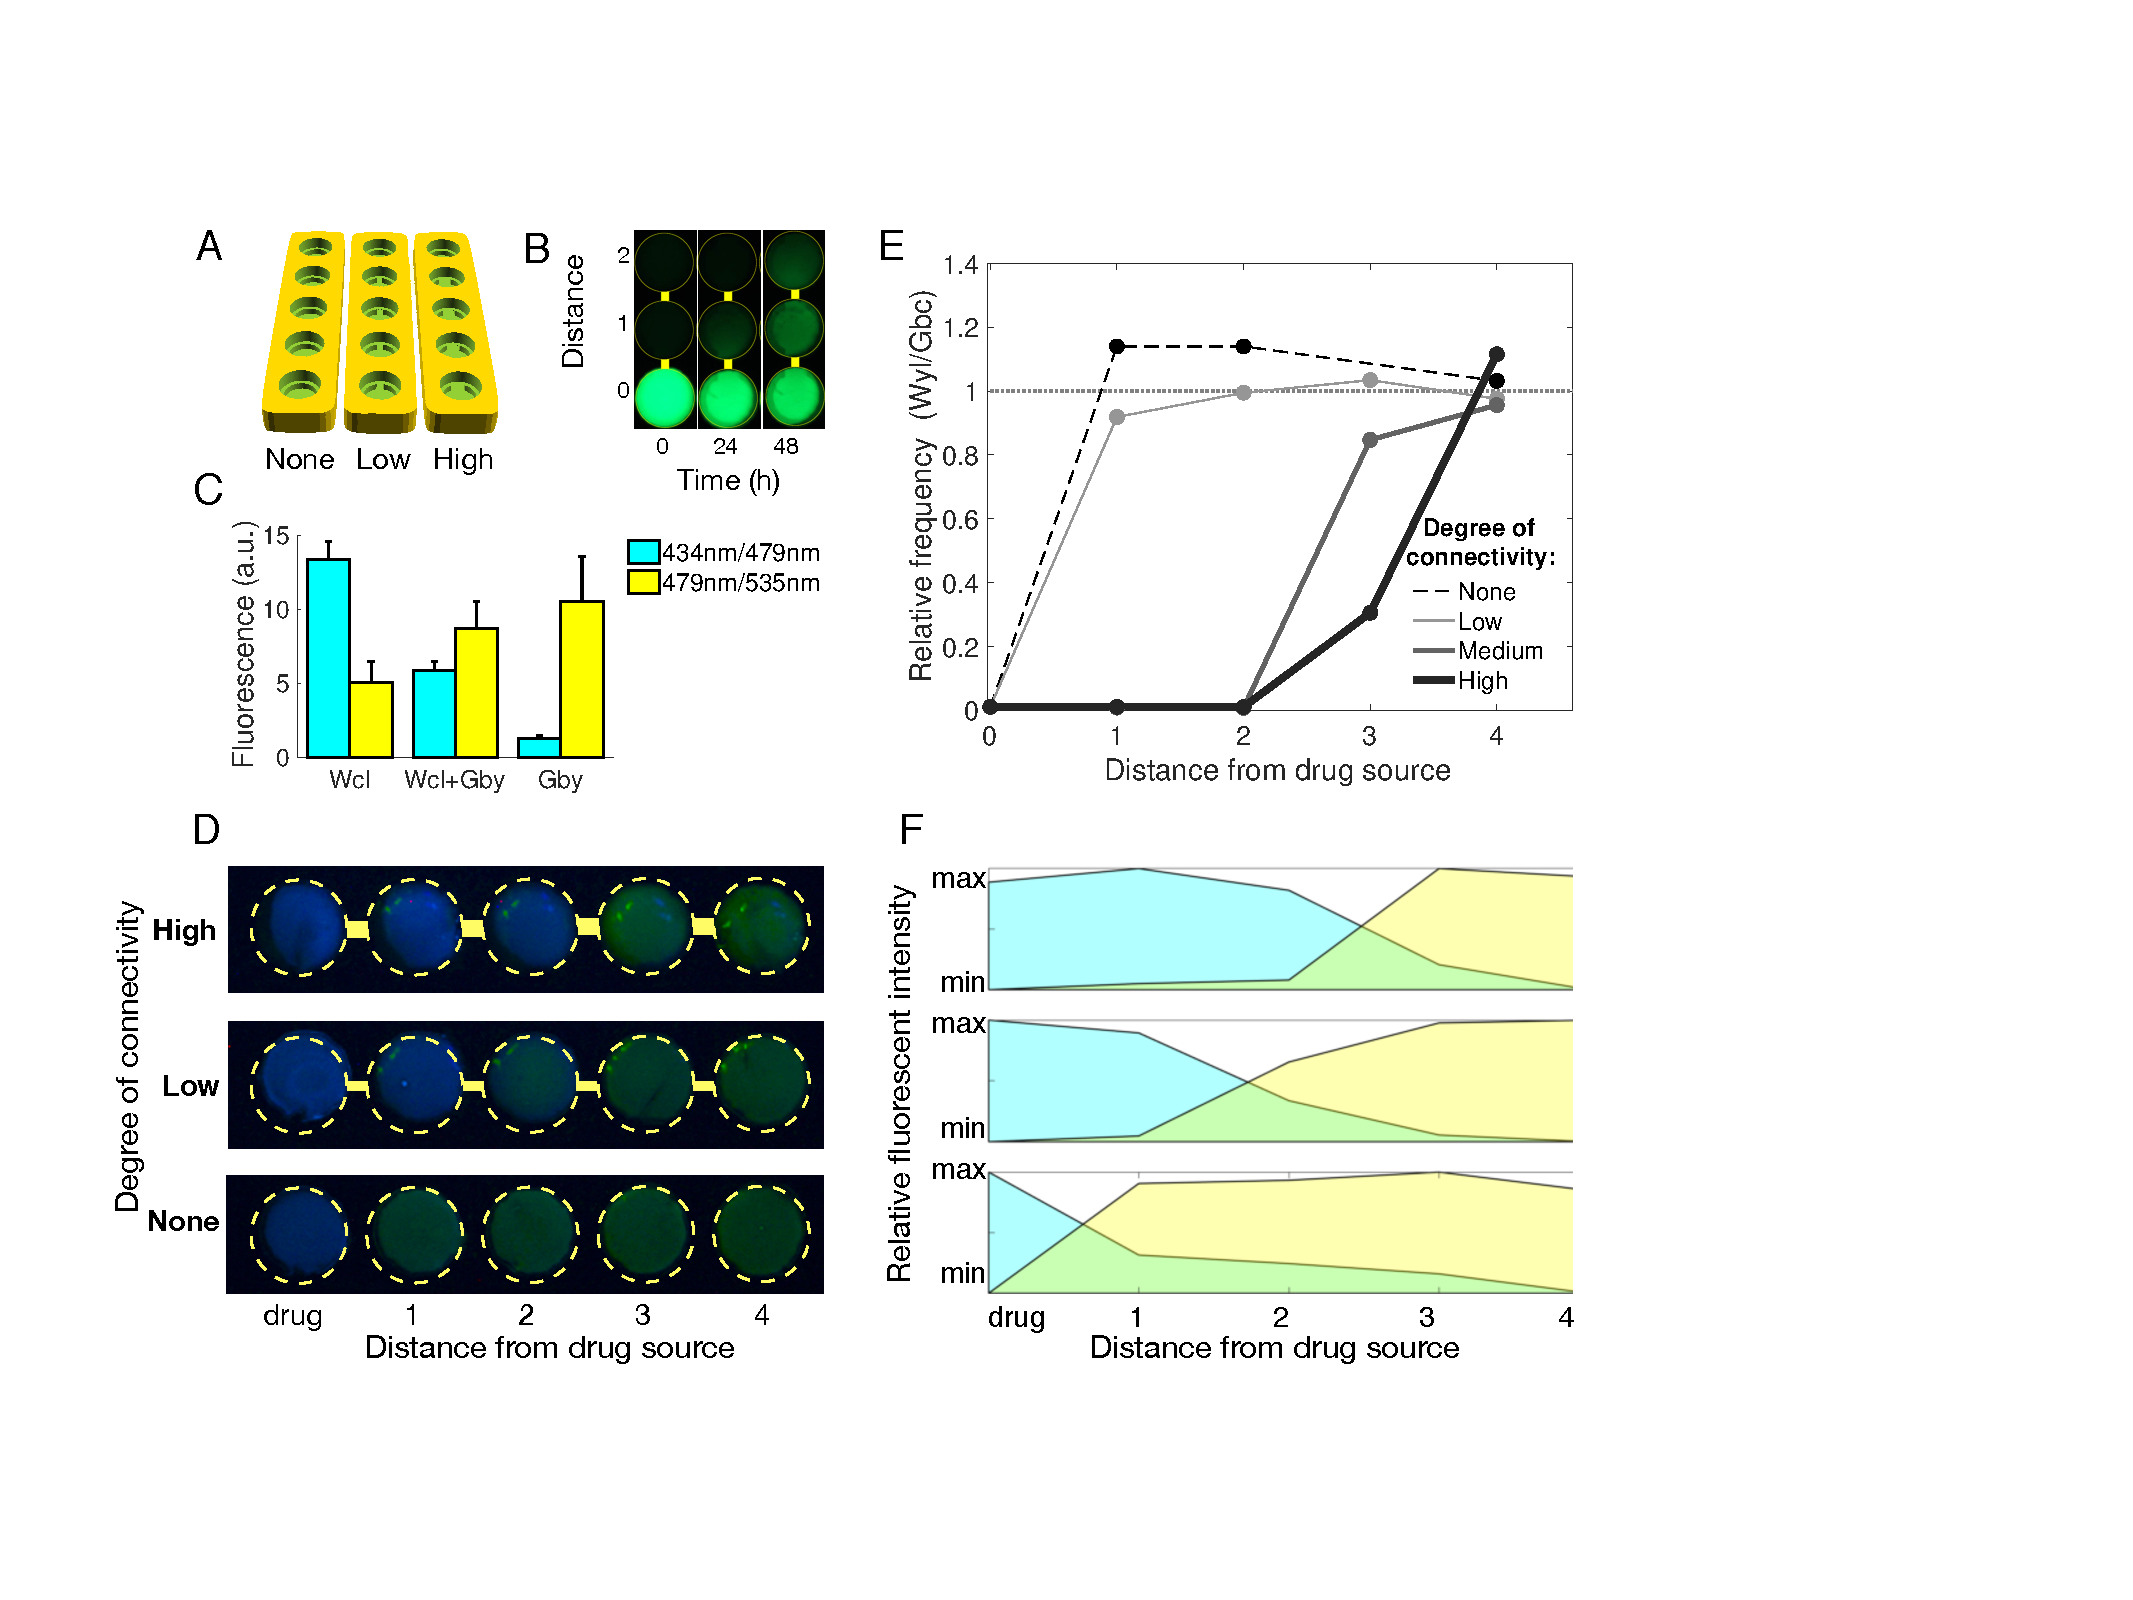
\includegraphics[width=.9\linewidth]{figures/Figure4.pdf}
\caption{\footnotesize Experimental results. A) CAD design of linear arrays of connected micro-environments with different degrees of connectivity. B) A gradient is formed after using a green fluorescent dye (pyranine) in the bottom compartment. Each column corresponds to a photograph of the device at different time-points.  C) Fluorescent intensity estimated using different fluorescence channels, both in mono-culture and in co-culture, of cells grown in the absence of antibiotics.  D) Growth of a mixed population after 24 hours in the devices depicted in A). Kanamycin is deployed in the left-most well and each well is inoculated with equal proportion of resistant and susceptible strains. The top two rows illustrate different channel widths between micro-environments (channels and well edges annotated with yellow lines), allowing the diffusion of antibiotic molecules between consecutive wells. Note how, as we increase connectivity, there are more wells whereby susceptible bacteria are outcompeted by the resistant strain (blue wells). The bottom row illustrates a control experiment where micro-environments are not connected, so the antibiotic is only present in the first well and therefore the remaining compartments are colonized by susceptible bacteria (yellow wells).   E) Relative frequency of susceptible bacteria (estimated using flow cytometry) observed in each micro-environment, as a function of the distance to the antibiotic source. F) Using image processing we estimated the relative fluorescence of each channel and validated the visible pattern observed in D); as the width of the channel increases, so does the number of compartments where the resistant strain (blue area) outcompetes the susceptible genotype (yellow area). }
\label{fig:figure4}
\end{figure}
%%%%%%%%

Figure \ref{fig:figure4}D shows a photograph taken after 24 hours using both CFP and YFP fluorescent channels; yellow compartments correspond to micro-environments where the susceptible subpopulation outcompeted resistant cells, and blue compartments where only resistant cells where observed. Using image analysis algorithms we obtained the relative fluorescent intensity of both channels (illustrated in Figure \ref{fig:figure4}F) and observed that, as predicted in the theoretical results shown in Figure \ref{fig:figure3}A, the width of the channel is correlated with the number of micro-environments where resistant cells have a higher fitness and outcompete the susceptible subpopulation.  

We recovered the bacteria from each well and centrifuged each sample into 1ml of liquid M9 without nutrients and used a flow cytometer to validate the fraction of cells in each subpopulation estimated using image analysis.  Indeed, Figure \ref{fig:figure4}E shows that in the low-connectivity regimes, the resistant subpopulation outcompetes susceptible bacteria in micro-environments near the drug source.  In contrast, when the connectivity is high, susceptible bacteria can grow in a reduced number of compartments.  

All together, we conclude that high connectivity between compartments in a linear array of micro-environments enhances diffusion of drug molecules, increasing the strength of selection in favour of drug resistance.  In the following section we will extend this model to consider complex networks of connected micro-environments.

%%%%%%%%%%%%

%%%%%%%%
%%Figure 5
\begin{figure}[ht!]
\centering
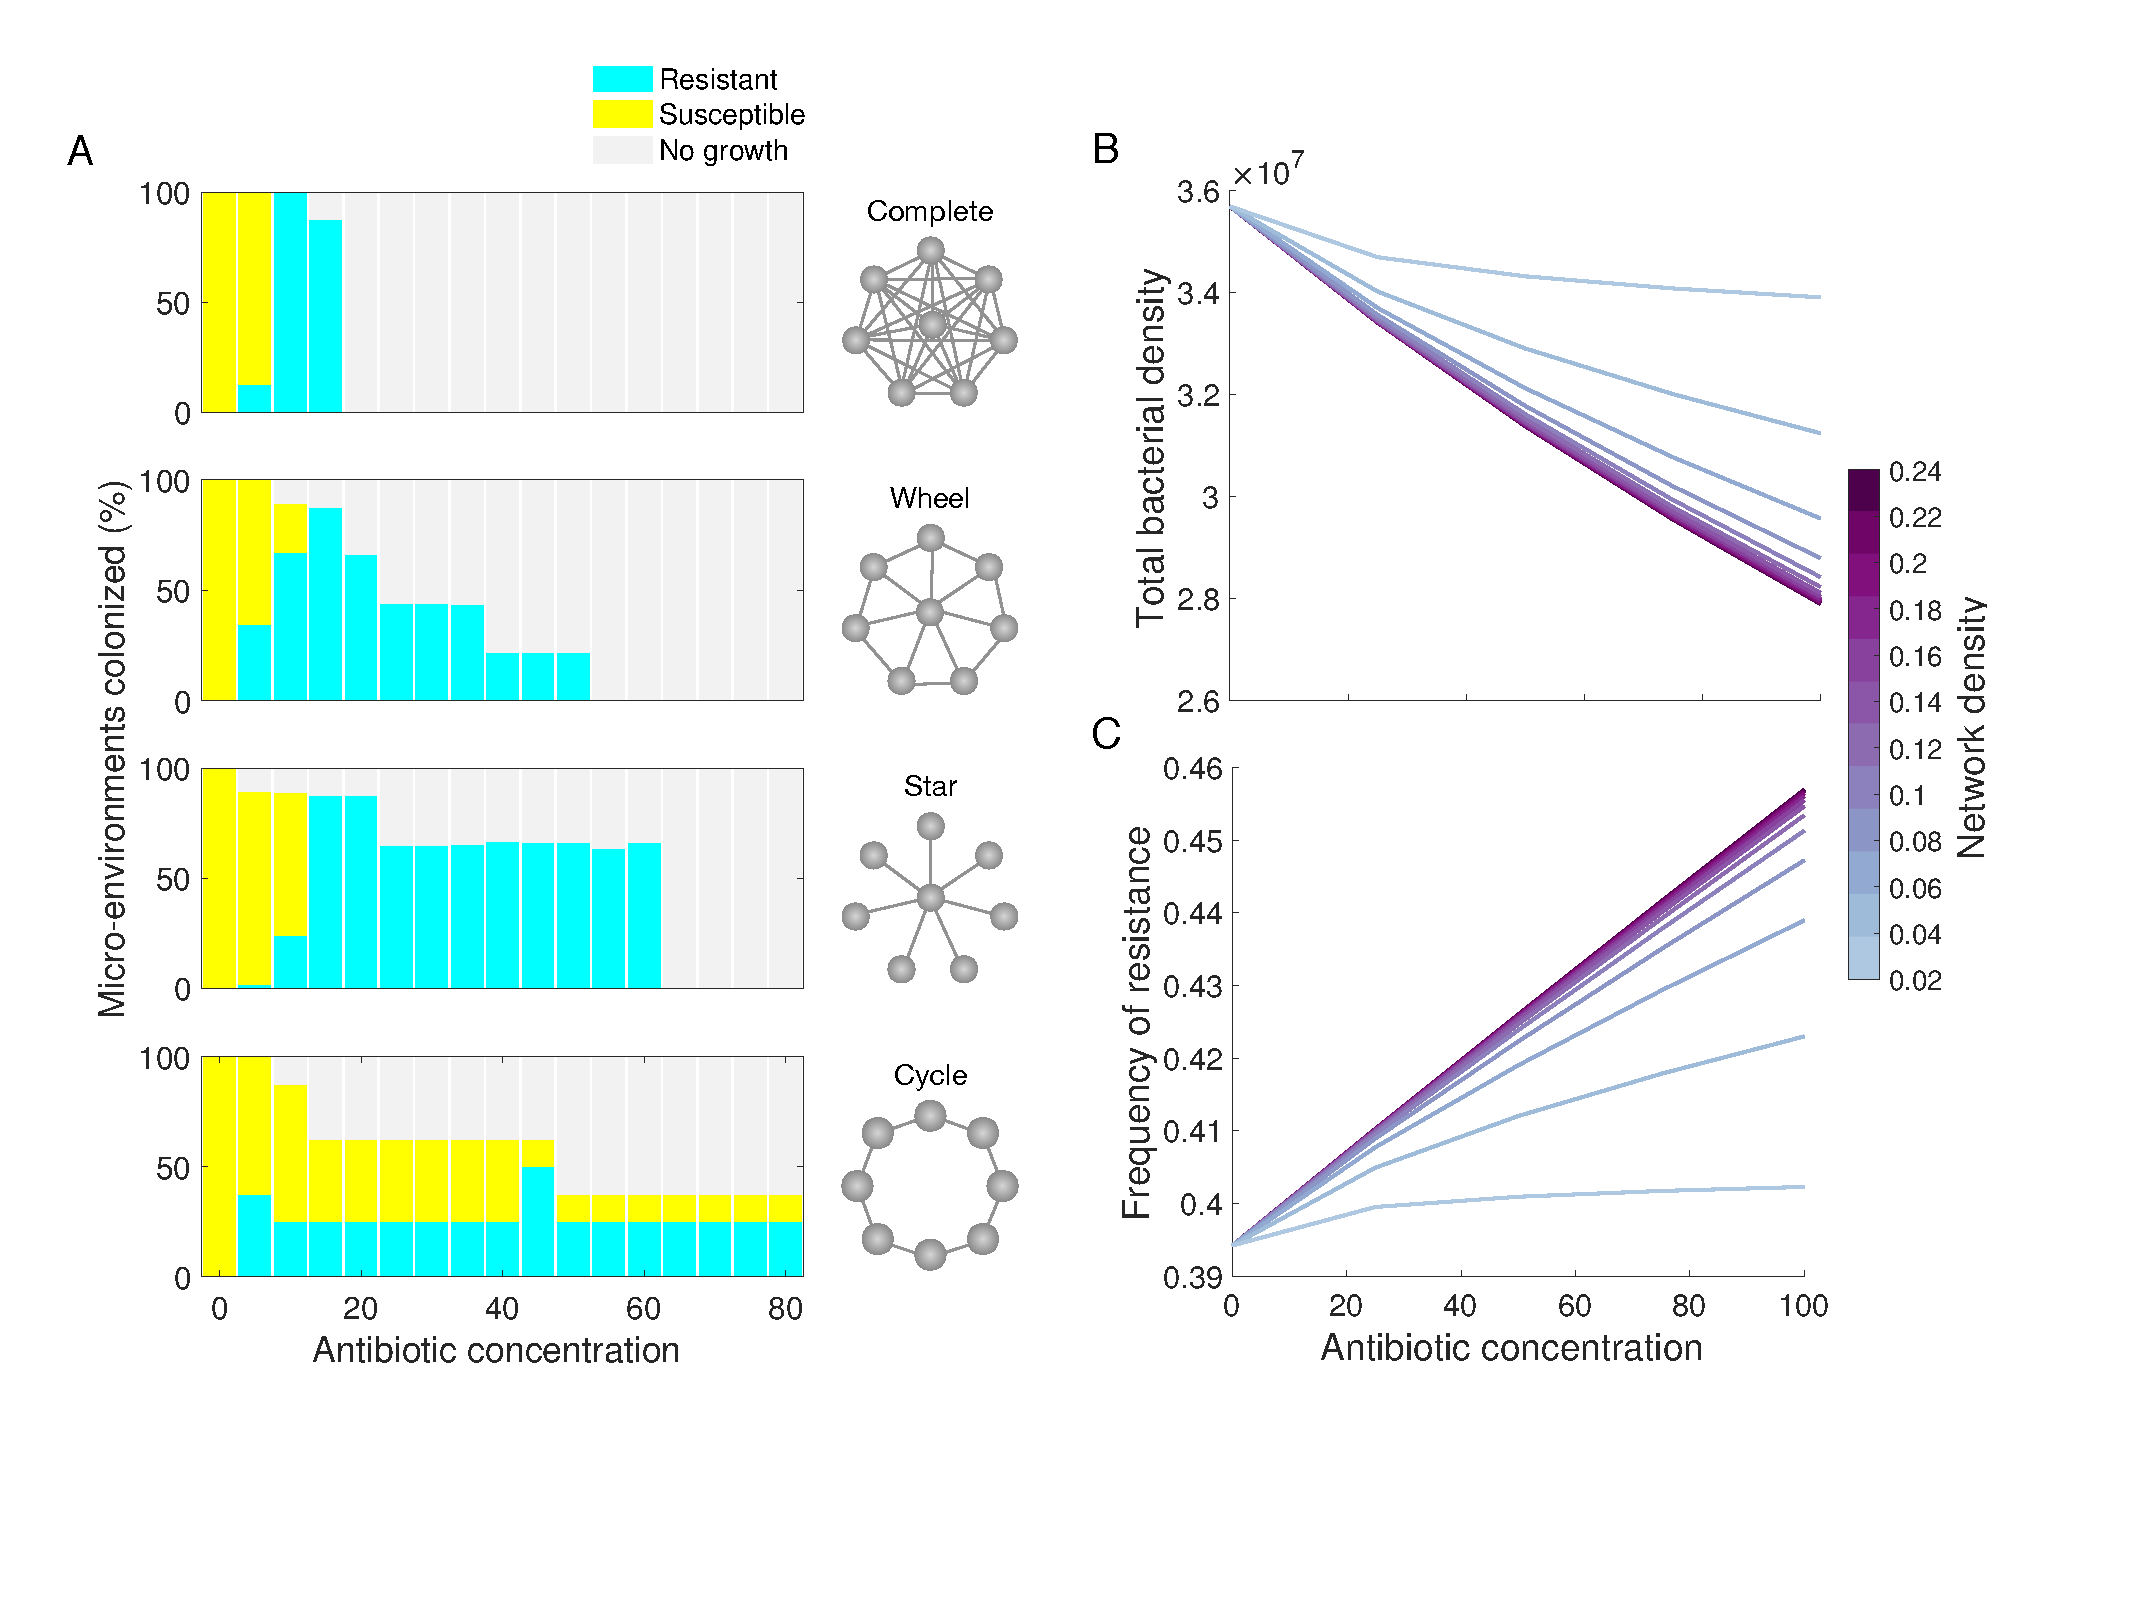
\includegraphics[width=1\linewidth]{figures/Figure5.pdf}
\caption{Numerical simulations of the population dynamics model in networks with different topological properties. Antibiotic is deployed in a random node of the network and allowed to diffuse to neighbouring micro-environments. A) Fraction of colonized micro-environments by each strain as a function of antibiotic concentration: cyan and yellow bars represent resistant and susceptible bacteria, respectively. Grey bars represent that no growth was detected at the end of the experiment. From top to bottom: complete, wheel, star and cyclical networks.  Note that networks with lower connectivity produce drug sanctuaries that allow for bacterial growth, even at high drug concentrations. B) Total bacterial density as a function of antibiotic concentration in random networks with different degrees of connectivity. We notice that bacterial density is negatively correlated with antibiotic concentration and network density. C) Frequency of resistance in the population is positively correlated with antibiotic concentration and network density.}
\label{fig:figure5}
\end{figure}
%%%%%%%%

\subsection*{Population dynamics in complex networks of connected micro-environments}

To explore the generality of the result presented previously, we now remove the constraint that micro-environments can only be connected linearly with a maximum of two neighbouring compartments.  As before, cells movement is not allowed but antibiotic molecules can diffuse between neighbouring compartments. We then use the population dynamics model presented in equations \ref{eq:ode}a-d to evaluate the effect of networks with different degrees of connectivity in the drug-resistance fitness landscape. Our goal is to count the nodes in the network where drug resistance is positively selected for, that is the fraction of the population locally exposed to drug concentrations within the mutant selection window.

First, we probed small networks with simple architectures and varying degrees of connectivity: a lattice, a star, a wheel and a complete network \cite{Askari2017}. We then introduced antibiotic in a random node of the network at $t=0$ and numerically solved the bacterial population dynamics model $T$ units of time, in order to estimate the total population density and the frequency of resistance of each node at $t=T$. It is important to notice that, while in the previous section we used the width of the channel to quantify the connectivity between two neighbouring nodes, we will now assume channel width between connected nodes is constant and focus on a topological definition of connectivity. For instance, we could define {\em network density} density based on the expression
${2m}/{n(n-1)},$
where $n$ and $m$ represent the number of nodes and edges of the network, respectively. Other measures that quantify the modularity of the network, for instance the network's clustering coefficient\cite{Opsahl2009}, produce qualitatively the same results. 

Figure 5A shows numerical results obtained after simulating $8000$ random networks under a range of antibiotic concentrations and parameter values described in Table 1. Each bar corresponds to the fraction of nodes in the network colonized by each strain (cyan and yellow for resistant and susceptible strains, respectively, and grey bars represent micro-environments where neither of the strains was able to grow).  In all cases, at low antibiotic concentrations, the susceptible strain colonized every micro-environment in the network.

%As expected, at intermediate drug concentrations we observe a mutant selection window whereby most micro-environments are colonized by the drug-resistant mutant.

Our results suggest that networks with high degree of connectivity (e.g. a complete graph) allow for a uniform distribution of antibiotics throughout every node in the graph, therefore effectively clearing both populations.  In contrast, in networks with intermediate connectivity (e.g. wheel and star), a gradient of antibiotics is produced and some micro-environments present drug concentrations within the mutant selection window, even if the antibiotic is deployed at concentrations higher than the mutant prevention concentration.  Interestingly, networks with low-connectivity (e.g. cycles), we observed drug sanctuaries where the antibiotic was present at very low concentrations, resulting in micro-environments colonized by susceptible bacteria. This is remarkable, given that the antibiotic was deployed at a very high dose.

Finally, in order to evaluate the evolutionary consequences of network topology on a large scale \cite{Allen2017}, we tested the population dynamics that emerges in random networks with different degrees of connectivity\cite{Watts1998}.  In particular, scale-free networks can be constructed algorithmically from the number of nodes $n$, the mean degree $k$ (an even integer) and a parameter $\beta$ satisfying $0 \leq \beta \leq 1$. We can then computationally obtain thousands of random undirected graph using the following recursive algorithm: first define a regular ring lattice with $n$ nodes, each connected to $k$ neighbors ($k/2$ on each side, with edges uniformly distributed among the nodes). Then, for node $n_i$, the edge $(n_i, n_j)$ with $i < j$ is randomly rewired with probability $\beta$ to any other node to which $n_i$ is not connected to. After producing each network, we estimated its density and simulated the population dynamics that emerges in response to a random node of the network receiving a lethal dose of antibiotics.

In Figures 5B and 5C we show results obtained after simulating ten thousand random networks of 100 nodes using different antibiotic concentrations. As expected, diffusion of antibiotics was increased in networks with higher density, resulting in a larger number of nodes with drug concentration above the mutant selection concentration.  Consequently, we found that total bacterial density decreased as a function of both network density and antibiotic concentration (Figure 5B).  As previously argued, this decrease in density is correlated, however, with an increased fraction of resistance in the population (Figure 5C). 

%%%%%%%%%%%%%%%%%%%%%%%%%%%%%%%%%%%%%%%%%%%
\section*{Discussion}

We presented a spatially-explicit population dynamics model to argue that diffusion of antibiotics in a heterogeneous environment maximally suppresses growth of a bacterial population.  Crucially, we also found that spatial regimes with enhanced diffusion also strengthen selection for antibiotic resistance and, as a result, increase the number of spatial locations with drug concentrations inside the mutant selection window. This prediction was corroborated by growing a co-culture of fluorescently-tagged susceptible and resistant strains in a 3D-printed gradient device and observing that the number of environments colonized by the resistant sub-population increased as a function of the connectivity between compartments.

Previous studies have established that spatial structure can drive bacterial communication \cite{Kim2016} and modulate diversity patterns in the population \cite{Rainey1998} and, in this context, it is not surprising that spatially-explicit environments can produce a heterogeneous spatio-temporal distribution of genotypes \cite{Legrand2017}. 
A limitation of our study is that we exclusively focused on the effect of drug gradients in the microbial population dynamics, while ignoring that the interaction between bacteria and environment can be mediated by other abiotic molecules. Indeed, previous theoretical and experimental studies have suggested that resource\cite{Mitri2015} and oxygen \cite{Chen2017} gradients can also have a central role in driving diversity patterns and shaping the spatial organization of microbial groups and their susceptibility to antimicrobial substances \cite{Sinclair2019}.  

Cell migration has also been reported to be a key driver of microbial evolutionary dynamics \cite{Baym2016,Okamoto2018}, for instance by allowing resistant cells to migrate upwards in an antibiotic gradient towards resource-rich regions where susceptible cells cannot survive. \cite{Hermsen2012}. 
It is important to highlight that we purposefully designed our culturing devices to allow diffusion of antibiotics through agar tunnels while blocking bacteria from moving between compartments. This compartmentalization of the environment is a coarse representation of the spatial structure found at multiple scales, from diverse tissue types in a single patient, to multiple patients in a hospital, to communities with different health trends.  Moreover, considering the environment as a series of locally-homogeneous micro-environments is consistent with our modelling assumptions, allowing us to use computer simulations to evaluate how, in the absence of migration, fitness landscapes change in time and space.

Another simplification of our study is that we artificially produced drug gradients by deploying antibiotics in a single location of the environment.  Then, by modifying the width of the channel that joins neighbouring compartments, we controlled the diffusion of antibiotic molecules between micro-environments. Of course, the antibiotic gradient achieved with our experimental protocol is a simplification of the complex profile of drug concentrations observed {\em in vivo} during antibiotic treatment. But we argue that the formation of antibiotic gradients is ubiquitous and that a uniform spatial distribution of drugs is impossible to achieve in practice. Actually, even if the initial distribution of antibiotics is homogeneous, antibiotic gradients can be self-generated from the interaction between the microbial population and the extracellular environment, for instance by the release of drug-degrading enzymes \cite{Yurtsev2013} or the absorption of antimicrobial molecules \cite{Snoussi2018}.  

A consequence of presenting a non-uniform spatial distribution of genotypes is that bacterial communities can implement collective strategies\cite{Pena2016} that would be evolutionary unstable in well-mixed environments, notably metabolic cross-feeding \cite{Pande2016},  production of signalling molecules \cite{Lee2010} and of extracellular matrix \cite{Nadell2017} that enable the formation of biofilms \cite{Flemming2016} and the implementation of population-based resistance mechanisms \cite{Lee2010,Estrela2018}.  Therefore we argue that spatial structure, being an inherent and unavoidable property of the environment, is not only key to understand the evolutionary forces driving drug resistance adaptation, but also potentially useful to decrease pathogenic virulence by disrupting quorum-sensing signalling \cite{Maeda2012,Kim2016} or in the design of spatially-targeted treatments that select against resistant genotypes \cite{Okamoto2018}.  


%%%%%%%%%%%%%%%%%%%%%%%%%%%%%%%%%%%%%%%%%%%
%%%%%%%%%%%%%%%%%%%%%%%%%%%%%%%%%%%%%%%%%%%

\section*{Materials and Methods}


%%%%%%%%%%%%
\subsection*{Bacterial strains and culture conditions}

For the competition assay between the resistant and susceptible bacteria to the antibiotic Kanamycin, we used two \textit{Escherichia coli} strains MC4100 \cite{Chait2007,Chait2010} labeled with either YFP (\textsc{Gby}) for the susceptible strain or CFP  (\textsc{Wcl}) for the resistant strain under a constitutive \textit{PLac} promoter. We also use MG1655 as a non-resistant, non-fluorescent control strain. All experiments were conducted using M9 \cite{} minimal media supplemented with $0.4\%$ of glucose and $0.2\%$ of casaminoacids.
Overnight cultures of \textsc{Wcl} and \textsc{Gby} strains were grown separately in M9 minimal media, as described above, at $30^{\circ}$ C in continuous shaking. After 20 hours of growth we measure optical density with a spectrophotometer and dilute the sample with the highest OD to equalize the optical density for both cultures. Then we make a mixture at 1:1 ratio, $10\mu$l of this co-culture is inoculated into each of the 96 well-plate with a range of Kanamycin dilutions in M9 minimal media at fixed doses, and incubated again at $30^{\circ}$ C for 20 hours. 
For the linear array assay we filled each well with $200 \mu l$ of soft M9 with nutrients as described above, for the fist well we add Kanamycin to the media ($50 \mu l/ml$) and let them dry and diffused at $4^ \circ$ C for 48 hours.  Then $10\mu l$ of bacterial culture (in a mixture at 1:1 ratio) was added to each well. The device was placed inside a petri dish, sealed with parafilm and incubated at $30^\circ$ C for 24 hours. 

%%%%%%%%%%%%
\subsection*{Fabrication of 3D-printed culture devices}

We used OpenScad to design culture devices composed of a linear array of micro-environments with different degrees of connectivity. Devices were fabricated using a commercial 3D printer (Robo3D R2) with polylactic acid (PLA). Each micro-environment and the channels that connect them were filled with semi-solid media (M9 + agar) allowing nutrients and antibiotic to move between neighbouring micro-environment by simple diffusion. Bacterial movement between micro-environments is prevented by independently inoculating the surface on each well with a 1:1 proportion of resistant and susceptible bacteria. CAD files for 3D printing can be downloaded from NIH 3D Print Exchange: \href{https://3dprint.nih.gov/discover/3dpx-011236}{https://3dprint.nih.gov/discover/3dpx-011236}.

%%%%%%%%%%%%
\subsection*{Flow cytometry}

To estimate relative abundances of each strain using flow cytometry, first we collected the bacterial population of each well by scraping all the surface and vortexing it in minimal media without nutrients to remove the agar.  We measured $10,000$ events per sample using CFP (7/405-175 mW) and YFP (2/488-150 mW) fluorescent channels of an Image Streamx Amnis flow cytometer. Analysis was performed using Image Stream Data Analysis and Exploration Software (IDEAS).

%%%%%%%%%%%%
\subsection*{Image acquisition and analysis}

We used image acquisition system engineered using low-cost, open-source software and hardware (based on Arduino microcontrollers, \href{http://www.arduino.cc/}{http://www.arduino.cc/}) and simple electronics components. This device controls a standard CCD camera (Canon EOS Rebel T6i with a $100$mm macro lens) and produces time-lapse movies from multi-channel images (each frame is an array of images acquired using different fluorescent channels, exposures times, etc). Fluorescence is quantified using high intensity LEDs (Luxeon Star, \href{http://www.luxeonstar.com/}{http://www.luxeonstar.com/}) and fluorescence imaging filters acquired from Thorlabs (Cyan: excitation $434 $nm and emission $479$ nm, and Yellow: excitation $497 $nm and emission $535$nm). Image analysis was performed using ImageJ (\href{https://imagej.nih.gov/ij/}{https://imagej.nih.gov/ij/}).  Design files and instructions to build the biological apparatus for fluorescence estimation used in this study can be downloaded from \href{https://github.com/ccg-esb-lab/baffle}{https://github.com/ccg-esb-lab/baffle}

%%%%%%%%%%%%
\section*{Acknowledgments}
We thank Arne Traulsen and Michael Sieber for useful discussions and for hosting AFM for a semester. We also thank Remy Chait for inspiration and for providing the strains used in this study. This work was supported by PAPIIT-UNAM grants 201016 and IN209419.

%%%%%%%%%%%%
\clearpage
\section*{Appendix}

\begin{center}
\captionof{table}{Parameters used in the numerical solutions of the population dynamics model \label{table:parameters}}
     \begin{tabular}{|c|c|l|} 
\hline
{\em Parameter} & {\em Value} & {\em Description} \\
\hline
\hline
$\delta_A$ &  $ 0.2 $ & antibiotic diffusion rate\\
$\delta_R$ &  $ 0.2 $ & resource diffusion rate\\
$\rho_*$ &  $ (1.4\times10^{8},1.05\times10^{8}) $ & resource conversion coefficient ($B_s$, $B_r$)\\
$\mu_*$ &  $ (7.3\times10^{-10},8\times10^{-10}) $ & maximum uptake rate ($B_s$, $B_r$)\\
$K_*$ &  $ (1,1) $ & half-saturation constant ($B_s$, $B_r$)\\
$\kappa_{1,*}$ &  $ (0.16,0.055) $ & affinity for antibiotic ($B_s$, $B_r$)\\
$\kappa_{2,*}$ &  $ (0.04,0.06) $ & maximal growth inhibition  ($B_s$, $B_r$)\\
$\alpha_*$ &  $ (10\times10^{-10},10\times10^{-9}) $ & antibiotic degradation rate ($B_s$, $B_r$)\\
\hline 
   \end{tabular}
\end{center}


%%%%%%%%%%%%%%%%%%%%%%%%%%%
\bibliography{refs}



\end{document}